\documentclass[12pt,letterpaper]{exam}
\usepackage[lmargin=1in,rmargin=1in,tmargin=1in,bmargin=1in]{geometry}
\usepackage{../style/exams}

% -------------------
% Course & Exam Information
% -------------------
\newcommand{\course}{MAT 100: Exam 1}
\newcommand{\term}{Fall -- 2022}
\newcommand{\examdate}{10/07/2022}
\newcommand{\timelimit}{85 Minutes}

\setbool{hideans}{false} % Student: True; Instructor: False

% -------------------
% Content
% -------------------
\begin{document}

\examtitle
\instructions{Write your name on the appropriate line on the exam cover sheet. This exam contains \numpages\ pages (including this cover page) and \numquestions\ questions. Check that you have every page of the exam. Answer the questions in the spaces provided on the question sheets. Be sure to answer every part of each question and show all your work.} 
\scores
%\bottomline
\newpage

% ---------
% Questions
% ---------
\begin{questions}

% Question 1
\newpage
\question[10] Showing all your work and finding an exact answer, compute the following:
	\begin{enumerate}[(a)]
	\item $3 (2^4) - 12$
	\item $\dfrac{(-2)^3 - 5 + 3 \cdot 6}{-5}$
	\item $\dfrac{5 \cdot 4 - 4 \cdot 3}{5 - 1}$
	\end{enumerate} \pspace

\sol
\begin{enumerate}[(a)]
\item 
	\[
	3 (2^4) - 12= 3(16) - 12= 48 - 12= 36
	\] \pspace

\item 
	\[
	\dfrac{(-2)^3 - 5 + 3 \cdot 6}{-5}= \dfrac{-8 - 5 + 3 \dot 6}{-5}= \dfrac{-8 - 5 + 18}{-5}= \dfrac{-13 + 18}{-5}= \dfrac{5}{-5}= -1
	\] \pspace

\item 
	\[
	\dfrac{5 \cdot 4 - 4 \cdot 3}{5 - 1}= \dfrac{20 - 12}{5 - 1}= \dfrac{8}{4}= 2
	\]
\end{enumerate}



% Question 2
\newpage
\question[10] Define the following sets:
	\[
	\begin{aligned}
	A&= \{ -3,\; 1, \; 2,\; 3,\; 5,\; 10,\; 20,\; 30,\; 40,\; 50 \} \\
	B&= \{ -3,\; 3,\; 10,\; 50 \} \\
	C&= \{ 2,\; 5,\; 20,\; 40,\; 50 \} \\
	D&= \{ -3,\; 1,\; 5 \} \\
	E&= \{ 1,\; 2,\; 3,\; 5 \}
	\end{aligned}
	\]
Consider all these sets as subsets of $A$. Compute the following:
	\begin{enumerate}[(a)]
	\item $D^c$
	\item $C \cup D$
	\item $B \setminus C$
	\item $D \cap E$
	\item $|E|$
	\end{enumerate} \pspace

\sol 
\begin{enumerate}[(a)]
\item 
	\[
	D^c=  \{ 2,\; 3,\; 10,\; 20,\; 30,\; 40,\; 50 \}
	\] \pspace

\item 
	\[
	C \cup D= \{ -3,\; 1,\; 2,\; 5,\; 20,\; 40,\; 50 \} 
	\] \pspace

\item 
	\[
	B \setminus C= \{ -3,\; 3,\; 10 \} 
	\] \pspace

\item 
	\[
	D \cap E= \{ 1,\; 5 \} 
	\] \pspace

\item 
	\[
	|E|= 4
	\]
\end{enumerate}



% Question 3
\newpage
\question[10] Determine whether the relation below is a function of not. Be sure to fully justify your response. If the relation is a function, find its domain, codomain, and range. 
	\[
	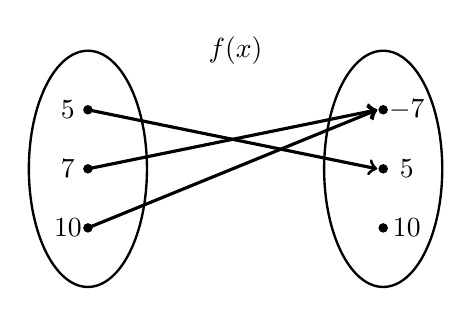
\begin{tikzpicture}[scale=0.75]
	\node at (2.5,2) {$f(x)$};
	% Ellipses
	\draw[line width=0.03cm] (0,0) circle (1 and 2);
	\draw[line width=0.03cm] (5,0) circle (1 and 2);
	
	% Nodes
	\draw[fill=black] (0,1) circle (0.07);
	\draw[fill=black] (0,0) circle (0.07);
	\draw[fill=black] (0,-1) circle (0.07);
	
	\draw[fill=black] (5,1) circle (0.07);
	\draw[fill=black] (5,0) circle (0.07);
	\draw[fill=black] (5,-1) circle (0.07);
	
	% Arrow
	\draw[line width=0.04cm,->] (0,1) -- (4.9,0);
	\draw[line width=0.04cm,->] (0,0) -- (4.9,1);
	\draw[line width=0.04cm,->] (0,-1) -- (4.9,1);
	
	% Labels
	\node at (-0.3,1) {$5\,$};
	\node at (-0.3,0) {$7\,$};
	\node at (-0.3,-1) {$10\,$};
	
	\node at (5.4,1) {$-7$};
	\node at (5.4,0) {$5$};
	\node at (5.4,-1) {$10$};
	\end{tikzpicture}
	\] \pspace

\sol {\itshape Because each input has a unique output, $f(x)$ is a function; that is, given any of the possible inputs---namely 5, 7, 10---we know the output---namely $f(5)= 5$, $f(7)= -7$, and $f(10)= -7$. The fact that $f(7)= -7$ and $f(10)= -7$ does not matter because the outputs need not be different from each other, only that the given the input, there is a unique output.} \pspace

{\itshape The domain of $f(x)$ is the set $\{ 5, 7, 10 \}$, the codomain of $f(x)$ is $\{ -7, 5, 10 \}$, and the range of $f(x)$ is $\{ -7, 5 \}$.}



% Question 4
\newpage
\question[10] Explain why $f(x, y)= x^2 - y + 1$ is a function. Then showing all your work, find $f(0, 0)$, $f(0, -4)$, $f(3, 6)$, and $f(-2, 10)$. \pspace

\sol {\itshape For each of the inputs, $(x, y)$, there is a unique output for $f(x, y)$, namely the one obtained by evaluating $f$ at $(x, y)$ and following order of operations. We have\dots} \pspace
	\[
	\begin{aligned}
	f(0, 0)&= 0^2 - 0 + 1= 0 - 0 + 1= 0 + 1= 1 \\[0.3cm]
	f(0, -4)&= 0^2 - (-4) + 1= 0 - (-4) + 1= 4 + 1= 5 \\[0.3cm]
	f(3, 6)&= 3^2 - 6 + 1= 9 - 6 + 1= 3 + 1= 4 \\[0.3cm]
	f(-2, 10)&= (-2)^2 - 10 + 1= 4 - 10 + 1= -6 + 1= -5
	\end{aligned}
	\]



% Question 5
\newpage
\question[10] Showing all your work, find the following:
	\begin{enumerate}[(a)]
	\item 56\% of 920
	\item 150\% of 60
	\item 1\% of 840
	\end{enumerate} \pspace

\sol 
\begin{enumerate}[(a)]
\item 
	\[
	920(0.56)= 515.2
	\] \pspace

\item 
	\[
	60(1.50)= 90
	\] \pspace

\item 
	\[
	840(0.01)= 8.40
	\]
\end{enumerate}



% Question 6
\newpage
\question[10] Showing all your work, compute the following:
	\begin{enumerate}[(a)]
	\item 150 increased by 42\%
	\item 245 decreased by 20\%
	\item 660 increased by 125\%
	\end{enumerate} \pspace

\sol 
\begin{enumerate}[(a)]
\item 
	\[
	150(1 + 0.42)= 150(1.42)= 213
	\] \pspace

\item 
	\[
	245(1 - 0.20)= 245(0.80)= 196
	\] \pspace

\item 
	\[
	660(1 + 1.25)= 660(2.25)= 1485
	\]
\end{enumerate}



% Question 7
\newpage
\question[10] Find the average value of the following numbers: $-7, -4.2, -1, 0, 2, 6, 10, 12$. \pspace

\sol {\itshape We have\dots}
	\[
	\begin{aligned}
	\text{Avg}(\{-7, -4.2, -1, 0, 2, 6, 10, 12\})&= \dfrac{\sum \text{ values}}{\# \text{ numbers}} \\[0.3cm]
	&= \dfrac{-7 + (-4.2) + (-1) + 0 + 2 + 6 + 10 + 12}{8} \\[0.3cm]
	&= \dfrac{17.8}{8} \\[0.3cm]
	&= 2.225
	\end{aligned}
	\]



% Question 8
\newpage
\question[10] Suppose a student's course grade consists of the following weights: \par
	\begin{table}[!ht]
	\centering
	\begin{tabular}{rrcrr}
	Homework & 40\% & & Exam 2 & 15\% \\
	Quizzes & 5\% & & Final Exam & 17\% \\
	Exam 1 & 8\% & & Project & 15\% \\
	\end{tabular}
	\end{table} \par
Suppose also that a student had a 85.6\% homework average, 80\% quiz average, 92\% on exam 1, 87\% on exam 2, 79\% on the final, and 95\% on the project. Compute the student's course average to the nearest tenth of a percent. \pspace

\sol {\itshape We have\dots}
	\[
	\begin{aligned}
	\text{Course Average}&= \sum \text{value} \cdot \text{weight} \\[0.3cm]
	&= 40\% (0.856) + 5\% (0.80) + 8\% (0.92) + 15\% (0.87) + 17\% (0.79) + 15\% (0.95) \\[0.3cm]
	&= 34.24 + 4.0 + 7.36 + 13.05 + 13.43 + 14.25 \\[0.3cm]
	&\approx 86.3\%
	\end{aligned}
	\] 



% Question 9
\newpage
\question[10] Suppose you take the courses shown below and receive the given letter grades. Showing all your work, compute your GPA to the nearest thousandth. The university's letter grade system is shown on the right below. \par
	\begin{table}[!ht]
	\centering
	\begin{tabular}{lrr}
	Course & Credits & Letter Grade \\ \hline
	Eastern Europe & 3 & B$-$ \\
	Modern American Literature & 3 & C$+$ \\
	Calculus~II & 4 & A\phantom{$-$} \\
	Chemistry~I & 4 & A$-$ \\
	Introduction to College Life & 1 & A\phantom{$-$} \\
	Freshman Seminar & 3 & B\phantom{$-$}
	\end{tabular} \hspace{1cm}
        \begin{tabular}{|l||c|l||c|} \hline
        A & 4.0 & C+ & 2.3 \\ \hline
        A-- & 3.7 & C & 2.0 \\ \hline
        B+ & 3.3 & C-- & 1.7 \\ \hline
        B & 3.0 & D & 1.0 \\ \hline
        B-- & 2.7 & F & 0.0 \\ \hline
        \end{tabular}
	\end{table} \pspace

\sol {\itshape We have\dots}
	\[
	\begin{aligned}
	\text{GPA}&= \dfrac{\sum \text{value} \cdot \text{credits}}{\text{total credits}} \\[0.3cm]
	&= \dfrac{2.7(3) + 2.3(3) + 4.0(4) + 3.7(4) + 4.0(1) + 3.0(3)}{3 + 3 + 4 + 4 + 1 + 3} \\[0.3cm]
	&= \dfrac{8.1 + 6.9 + 16 + 14.8 + 4 + 9}{18} \\[0.3cm]
	&= \dfrac{58.8}{18} \\[0.3cm]
	&\approx 3.267
	\end{aligned}
	\]



% Question 10
\newpage
\question[10] Showing all your work, convert 648~in$^2$ to square feet. Recall that there are twelve inches in every foot. \pspace

\sol {\itshape We have\dots \par}
	\begin{table}[!ht]
	\centering
	\begin{tabular}{r|r|r}
	648 in$^2$ & 1~ft & 1~ft \\ \hline
			& 12~in & 12~in
	\end{tabular}
	= 4.5~ft$^2$
	\end{table}



% Question 11
\newpage
\question[10] Showing all your work, convert 9.5~km/hr to feet per minute. Note that 1~m is 3.28084~ft. \pspace

\sol {\itshape We have\dots}
	\begin{table}[!ht]
	\centering
	\begin{tabular}{r|r|r|r}
	9.5~km & 1000~m & 3.28084~ft & 1~hr \\ \hline
	1~hr & 1~km	     & 1~m           & 60~min
	\end{tabular}
	= 519.466~ft/min
	\end{table}



% Question 12
\newpage
\question[10] Suppose you are covering a wall with black and white checker tiles. The wall measures 40~ft across and is 9~ft tall. If each tile is 6~in by 6~in, how many tiles will you need to cover the wall? Suppose also that you can put tiles on the wall at a rate of 3~tiles per minute. How long will it take you to tile the wall? For both questions, be sure to show all your work and fully justify your answer. \pspace

\sol {\itshape Note that it takes 2~tiles to cover a 1~ft wide area. Then it will require $2 \cdot 40= 80$~tiles to cover the width of the wall. However, this line of tiles only covers up to a height of 6~in. Another layer, requiring an additional 80~tiles for a total of $80 + 80= 160$~tiles, will cover the width up to 1~ft high. Another 8~ft, i.e. 8~layers, will then cover the entire wall. This will then use an additional $8 \cdot 160= 1280$~tiles for a total of $160 + 1280= 1440$~tiles, i.e.  720~black tiles and 720~white tiles. Alternatively, the area of the wall is $A= lw= 40 \text{ ft} \cdot 9 \text{ ft}= 360 \text{ ft}^2$. Each tile is 6~in by 6~in, i.e. 0.5~ft by 0.5~ft. The area of each tile is then $(0.5 \text{ ft})(0.5 \text{ ft})= 0.25 \text{ ft}^2$. Therefore, it will take $360 \text{ ft}^2/ 0.25 \text{ ft}^2= 1440 \text{ tiles}$, i.e. 720~black tiles and 720~white tiles. \pspace

To find the total amount of time required to tile the wall, we have that we tile at a rate of 3~tiles per minute with a total of 1,440~tiles to place. This will require $1440 \text{ tiles}/(3 \text{ tiles/min})= 480 \text{ min}$, i.e. 8~hours. }



% Question 13
\newpage
\question[10] Showing all your work, find the volume of a cylinder that is measures 4~in across the bottom and is 11~in tall. \pspace

\sol {\itshape Note that because the cylinder measures 4~in across the entire bottom, its diameter is 4~in. But then the radius of the cylinder is 2~in. The height is 11~in. But then we have\dots
	\[
	V= \pi r^2 h= \pi (2 \text{ in})^2 \cdot 11 \text{ in}= pi \cdot 4 \text{ in}^2 \cdot 11 \text{ in}= 44\pi \text{ in}^3 \approx 138.23 \text{ in}^3
	\]
}



% Question 14
\newpage
\question A city is laid out in a grid structure with street corners meeting at right angles, as shown below with the street labeled. Suppose you are standing at point $P$ and your friend is standing at point $Q$.
	\[
	\fbox{%
	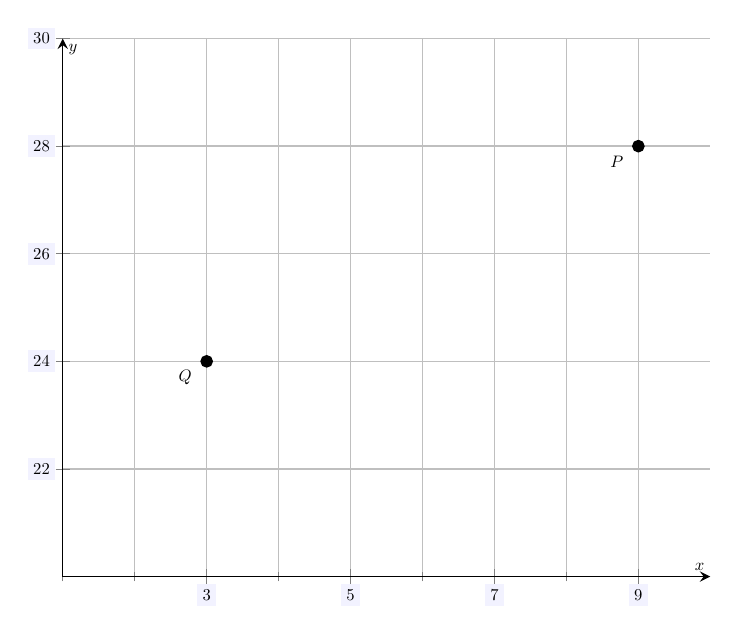
\begin{tikzpicture}[scale=1.2,every node/.style={scale=0.5}]
	\begin{axis}[
	grid=both,
	axis lines=middle,
	ticklabel style={fill=blue!5!white},
	xmin= 1, xmax=10,
	ymin= 20, ymax=30,
	xtick={1,3,5,7,9},
	ytick={20,22,24,26,28,30},
	minor tick = {-8,-7,...,8},
	xlabel=\(x\),ylabel=\(y\),
	]
	\node at (2.7,23.7) {$Q$};
	\draw[fill=black] (3,24) circle (0.06cm);
	\node at (8.7,27.7) {$P$};
	\draw[fill=black] (9,28) circle (0.06cm);
	\end{axis}
	\end{tikzpicture}
	}
	\]
\begin{parts}
\part[4] How many blocks are you from your friend `as the crow flies'?
\part[4] How many blocks are you from your friend using the taxicab metric?
\part[2] Supposing you can walk a block in 4~min and given your answer in (b), how long do you estimate that it will take you to walk to your friend?
\end{parts} \pspace

\sol {\itshape
\begin{enumerate}[(a)]
\item This is the Euclidean distance from $P$ to $Q$:
	\[
	\sqrt{(3 - 9)^2 + (24 - 28)^2}= \sqrt{(-6)^2 + (-4)^2}= \sqrt{36 + 16}= \sqrt{52} \approx 7.21 \text{ blocks}
	\] \pspace

\item Using the taxicab/Manhattan metric, we have\dots
	\[
	|3 - 9| + |24 - 28|= |-6| + |-4|= 6 + 4= 10 
	\] \pspace

\item Given that we are in a city, the taxicab/Manhattan metric seems to be the more useful metric of distance. By (b), we are a total 10~blocks from our friend by (b). We walk a block in 4~min, i.e. we walk at a pace of 4~min/block. But then, it should take approximately $10 \text{ blocks} \cdot 4 \text{ min}/\text{block}= 40$~minutes to walk to our friend. 
\end{enumerate}
}



% Question 15
\newpage
\question[10] Showing all your work and fully explaining your approximation, estimate how many pet dogs there are in the United States. \pspace

\sol {\itshape Answers will vary, but here is a possible approach: \pspace

I approximate from my own experience that about 1 in every 10 people that I know own a dog. They typically own one dog but occasionally they will own two or three. I then estimate that of the 1 in 10 people that own a dog, they own 1.5~dogs on average. The population of the United States is approximately 330~million. Therefore, the estimated amount of pet dogs in the United States is then\dots
	\[
	\dfrac{1}{10} \cdot 330000000 \cdot 1.5= 49,500,000
	\]
}


\end{questions}
\end{document}